\documentclass[10pt,twocolumn]{article}
\usepackage[a4paper, total={7in, 10in}]{geometry}
\usepackage{times}
\usepackage{graphicx}
\usepackage{amsmath}
\usepackage{enumitem}
\usepackage{titlesec}
\usepackage{fancyhdr}
\usepackage{hyperref}
\usepackage{caption}
\usepackage{float}
\usepackage{cite}
\usepackage[vietnamese]{babel}

\pagestyle{fancy}
\fancyhf{}
\rhead{ICT Research and Applications}
\lhead{Vol. 2025, No. 1, April}
\cfoot{\thepage}

\title{\textbf{\LARGE BUILDING A DEEP LEARNING-BASED TEXT SUMMARIZATION MODEL}}
\author{
Hoang Bao Viet, 
Nguyen Huyen Trang, 
Nguyen Thi Ha Phuong \\
The University of Danang, Vietnam - Korea University of Information and Communication Technology
}

\date{}

\begin{document}
\twocolumn[
\maketitle
\vspace{-2em}


\vspace{1em}
\begin{abstract}
Automatic text summarization is an important task in Natural Language Processing (NLP). This paper proposes a deep learning-based text summarization model for Vietnamese using the Transformer architecture. The model is trained on Vietnamese news datasets and evaluated using the ROUGE metric. Experimental results demonstrate that the proposed approach outperforms traditional summarization methods.
\end{abstract}

\textbf{Keywords:} text summarization, deep learning, Transformer, NLP, Vietnamese
\vspace{1em}
]

\section*{I. INTRODUCTION}
The vast amount of online content today leads to an increasing demand for automatic text summarization to help users quickly grasp the main ideas of long documents. Automatic summarization techniques can significantly enhance information processing in digital environments.

\vspace{1em}
\section*{II. RELATED WORKS}
Recent approaches such as BART, T5, and Pegasus have shown promising results in abstractive summarization. However, applications for the Vietnamese language still face challenges due to limited datasets and linguistic complexity.

\vspace{1em}
\section*{III. PROPOSED METHOD}
Our proposed model includes:

\begin{itemize}[noitemsep]
  \item Text pre-processing
  \item Encoder using Transformer layers
  \item Decoder generating the summary
\end{itemize}

\begin{figure}[H]
\centering
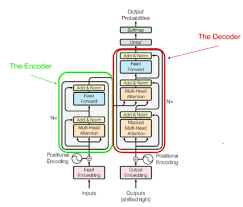
\includegraphics[width=0.45\textwidth]{img/imagesAttention.png}
\caption{The architecture of the proposed summarization model}
\end{figure}

\vspace{1em}
\section*{IV. EXPERIMENTS}
We use a dataset composed of Vietnamese news articles from sources like VnExpress and ZingNews. Evaluation is conducted using ROUGE-1, ROUGE-2, and ROUGE-L metrics.

\begin{table}[H]
\centering
\caption{Evaluation results of the model}
\begin{tabular}{|c|c|c|c|}
\hline
\textbf{Model} & \textbf{ROUGE-1} & \textbf{ROUGE-2} & \textbf{ROUGE-L} \\
\hline
TF-IDF + LSA & 38.2 & 17.3 & 35.0 \\
Proposed Transformer & \textbf{52.5} & \textbf{26.1} & \textbf{48.3} \\
\hline
\end{tabular}
\end{table}

\vspace{1em}
\section*{V. CONCLUSION}
This paper presents a Transformer-based model for Vietnamese text summarization. The model achieves promising results, offering a solid foundation for further research in Vietnamese NLP.

\vspace{1em}
\section*{ACKNOWLEDGMENT}
This research is supported by Vietnam - Korea University of Information and Communication Technology and the VKU AI Research Group.

\vspace{1em}
\section*{REFERENCES}
\begin{enumerate}[label={[{\arabic*}]}]
\item Vaswani et al., ``Attention is All You Need'', NeurIPS, 2017.
\item Raffel et al., ``T5: Exploring the Limits of Transfer Learning'', JMLR, 2020.
\item Nguyen T. H. et al., ``PhoBERT: Pre-trained language models for Vietnamese'', EMNLP, 2020.
\item Lin, C. Y., ``ROUGE: Recall-Oriented Understudy for Gisting Evaluation'', 2004.
\end{enumerate}

\end{document}
